\chapter{Design and Implementation}
\label{bab:4}

This chapter describes how PeerToCP is designed and built. It introduces the libraries and frameworks it uses and why they were chosen, the design of the system and how it is used, how each of the three variants keeps its replicas consistent, and finally the test scenarios used to compare them.

\section{Libraries and Frameworks}

PeerToCP builds on several third-party libraries, each chosen for a specific reason. The base of the desktop application is Electron. Figure~\ref{fig:4:components} shows how the components described in this section fit together in one PeerToCP client.

\begin{figure}[htbp]
    \centering
    % The components of one PeerToCP client (an Electron app): the renderer
% process with the editor, the shared state and the shell windows; the main
% process with the compiler and node-pty; and the network provider, one per
% variant. TikZ libraries: arrows.meta. Colors from thesis.sty.
\begin{tikzpicture}[
  font=\sffamily\footnotesize,
  proc/.style={draw=accent, line width=0.8pt, rounded corners=3pt, fill=white},
  frame/.style={draw=rulegray, line width=0.6pt, rounded corners=4pt},
  title/.style={font=\sffamily\small\bfseries, text=accent, anchor=west, inner sep=0pt},
  comp/.style={draw=black!60, line width=0.6pt, rounded corners=2pt, fill=white,
    align=center, inner sep=2pt, minimum height=0.85cm},
  alt/.style={draw=black!60, line width=0.6pt, rounded corners=2pt, fill=white,
    dash pattern=on 3pt off 2pt, align=center, inner sep=2pt},
  both/.style={line width=0.6pt, {Stealth[length=2.2mm,width=1.6mm]}-{Stealth[length=2.2mm,width=1.6mm]}},
  one/.style={line width=0.6pt, -{Stealth[length=2.2mm,width=1.6mm]}},
  lab/.style={font=\sffamily\footnotesize, inner sep=1.5pt},
]
  % ---- the client --------------------------------------------------------
  \draw[frame] (0,0) rectangle (15.8,-5.8);
  \node[title, text=black!70] at (0.2,-0.3) {PeerToCP client (Electron app)};

  % ---- renderer process ----------------------------------------------------
  \draw[proc] (0.2,-0.6) rectangle (9.9,-5.55);
  \node[title] at (0.4,-0.9) {Renderer process (Chromium)};
  \node[comp, text width=2.4cm] (cm) at (1.725,-2.6) {CodeMirror~6\\editor};
  \node[comp, text width=2.4cm] (xt) at (1.725,-3.65) {\texttt{xterm.js}\\shell windows};
  % shared state
  \draw[draw=accent, line width=0.6pt, fill=accentlight, rounded corners=3pt]
    (5.7,-1.2) rectangle (9.7,-5.35);
  \node[title, font=\sffamily\footnotesize\bfseries] at (5.85,-1.45) {Shared state};
  \draw[draw=black!60, line width=0.6pt, fill=white, rounded corners=2pt]
    (5.85,-1.7) rectangle (9.55,-4.25);
  \node[anchor=west, inner sep=0pt] at (6.0,-1.95) {Yjs \texttt{Y.Doc} (CRDT variants)};
  \node[comp, minimum width=3.4cm] (ytext) at (7.7,-2.6) {\texttt{Y.Text}\\the code};
  \node[comp, minimum width=3.4cm] (ymap) at (7.7,-3.65) {\texttt{Y.Map} of \texttt{Y.Array}\\the shells};
  \node[alt, minimum width=3.7cm] (collab) at (7.7,-4.8)
    {or, in the OT variant:\\[-1pt]\texttt{@codemirror/collab}};
  % bindings
  \draw[both] (cm) -- (ytext);
  \node[lab, above] at (4.35,-2.6) {\texttt{y-codemirror.next}};
  \draw[both] (xt) -- (ymap);

  % ---- main process ----------------------------------------------------------
  \draw[proc] (10.9,-0.6) rectangle (15.6,-3.9);
  \node[title] at (11.1,-0.9) {Main process (Node.js)};
  \node[comp, text width=4.2cm, minimum height=0.6cm] (gpp) at (13.25,-1.6)
    {system compiler (\texttt{g++})};
  \node[comp, text width=4.2cm] (pty) at (13.25,-3.0)
    {\texttt{node-pty}\\[-1pt]spawns programs in pseudoterminals};
  \draw[one] (gpp) -- node[lab, right] {executable} (pty);
  \node[comp, text width=4.2cm, minimum height=0.6cm, fill=codebg] (prog) at (13.25,-5.15)
    {compiled program};
  \draw[both] (pty) -- node[lab, right] {spawns; I/O} (prog);
  % renderer <-> main
  \draw[both] (9.9,-2.25) -- node[lab, above] {IPC} (10.9,-2.25);

  % ---- network provider -------------------------------------------------------
  \draw[frame, draw=black!60] (0,-6.4) rectangle (15.8,-8.6);
  \node[title, text=black!70] at (0.2,-6.68) {Network provider (one per variant)};
  \foreach \plib/\pdest/\pvar [count=\i] in {
      y-webrtc/{other peers (WebRTC data channels; WebSocket to the signaling server)}/peer-to-peer CRDT,
      y-websocket/{server (WebSocket)}/client-server CRDT,
      rpc-websockets/{OT server (WebSocket RPC)}/client-server OT} {
    \pgfmathsetmacro{\y}{-7.17-0.5*(\i-1)}
    \node[anchor=west, inner sep=0pt, font=\ttfamily\footnotesize\bfseries, text=accent] at (0.4,\y) {\plib};
    \draw[one] (2.75,\y) -- (3.35,\y);
    \node[anchor=west, inner sep=0pt] at (3.5,\y) {\pdest};
    \node[anchor=east, inner sep=0pt, font=\sffamily\footnotesize\itshape, text=black!60] at (15.6,\y) {\pvar};
  }
  \draw[rulegray, line width=0.4pt] (0.4,-7.42) -- (15.6,-7.42);
  \draw[rulegray, line width=0.4pt] (0.4,-7.92) -- (15.6,-7.92);
  % shared state <-> provider
  \draw[both, accent, line width=1pt] (7.7,-5.35) -- node[lab, right, text=accent] {updates} (7.7,-6.4);
\end{tikzpicture}%

    \caption[The components of a PeerToCP client]{The components of a PeerToCP client. The renderer process holds the editor and the shared state; the main process compiles and runs programs; the network provider, which differs between the variants, connects the client to its peers or to the server.}
    \label{fig:4:components}
\end{figure}

\subsection{Main Framework and Code Editor Component}

Electron is a framework for desktop applications that are built like web applications. Its user interface is rendered by Chromium, from HTML (HyperText Markup Language), CSS (Cascading Style Sheets) and JavaScript, and its back end runs on Node.js~\citep{kredpattanakul2018transforming, miglanielectron}, a JavaScript runtime built on Google's V8 engine~\citep{tilkov2010node}.

Electron applications are cross-platform: they run on Windows, GNU/Linux and macOS. Electron gives access to many operating system functions, such as spawning subprocesses and writing files. Because its front end is written with web technologies, an Electron application is also comparatively easy to port to the web, with its functionality limited to what the web allows. Alternatives include Qt, based on C++, and Tauri, based on Rust. Electron was chosen because widely used libraries for operational transformation, CRDTs, WebSocket and WebRTC already exist in JavaScript and can be used directly from Node.js.

An Electron application has a main process that runs when the application starts~\citep{electron}, and each window it opens is a renderer process. The main PeerToCP window is a code editor. Its renderer process can communicate with the main process at any time, and it opens the shell windows in which compiled programs run. The renderer process renders the front end, much like a web page. The central component of the main window is CodeMirror.

CodeMirror is the code editor component, and the user's main point of interaction with the application. It runs in a web browser and models text with an immutable state and modular change operations. It offers many extensions, good accessibility and support for many programming languages. CodeMirror is also the bridge to Yjs, the CRDT library, which already has a CodeMirror binding.

\subsection{Collaboration Components}

Yjs is a library that implements the YATA (Yet Another Transformation Approach) CRDT~\citep{Nicolaescu2016yjs}. Its core is the shared document, \texttt{Y.Doc}, which holds the CRDT data structures: \texttt{Y.Text} for text, and \texttt{Y.Map} and \texttt{Y.Array}, which PeerToCP combines to store the shells and their history. This study uses all three, each with its own abstraction.

Yjs is not tied to a particular network architecture. This study uses two network providers that connect a \texttt{Y.Doc} to other replicas: y-webrtc, for a full-mesh peer-to-peer network, and y-websocket, for a client-server network. Yjs has many active developers and was still being maintained and developed, which is why it was chosen for this study.

For the operational transformation variant, PeerToCP uses @codemirror/collab, CodeMirror's collaborative editing extension. Its network provider, for the client-server architecture, uses a modified rpc-websockets library that supports broadcasting, messaging a specific client, and asynchronous, non-blocking, promise-based remote procedure calls (RPC).

In the OT variant, to keep the program simple, a shell is stored as an append-only array, following OT principles. The operations on a shell are the users' keystrokes. Keystrokes are passed to the terminal as they are, and the program running in the shell decides how to interpret them. A backspace on the shell's input, for example, is recorded by default as the three characters ``$\texttt{\char`\\ b \char`\\ b}$'' (without the quotes): move the cursor left, write a space and move the cursor left again. To collaborate on a shell, every client sends its keystrokes into one shared input channel, without the separate cursors of the code editor.

\subsection{Shell Component}

A shell that runs programs, and that every client in the network can use, needs a library with access to the operating system, to compile and run code. Compilation converts code in a higher-level, human-readable language into binary code a machine can execute~\citep{aho1985compilers}. Besides editing code together, every user can compile a single-file program, using a compiler installed on their operating system. In Node.js, the library that gives access to it is node-pty.

node-pty is a Node.js library that forks processes attached to pseudoterminals. It streams data to and from a process managed by the operating system, and PeerToCP uses it to run compiled command-line (CLI) programs, which have no graphical user interface. It was chosen because it is widely used and cross-platform. The shell also needs a front end, for which PeerToCP uses xterm.js, a component that displays a terminal on a web page. xterm.js takes input from the browser and displays output, and it can be connected to a process running on the system. It has no dependencies, which is why it was chosen.

\section{System Design}

PeerToCP is a desktop application, which runs directly on the user's computer. This makes offline use easier, since no internet connection is needed to open it. Compiling on a peer also needs access to system calls, which web browser APIs do not provide~\citep{v8, spidermonkey}: browsers are designed this way so that scripts cannot attack the computer's operating system directly. Figure~\ref{fig:4:app} shows the application, and Figure~\ref{fig:activity} outlines how it is used.

\begin{figure}[htbp]
    \centering
    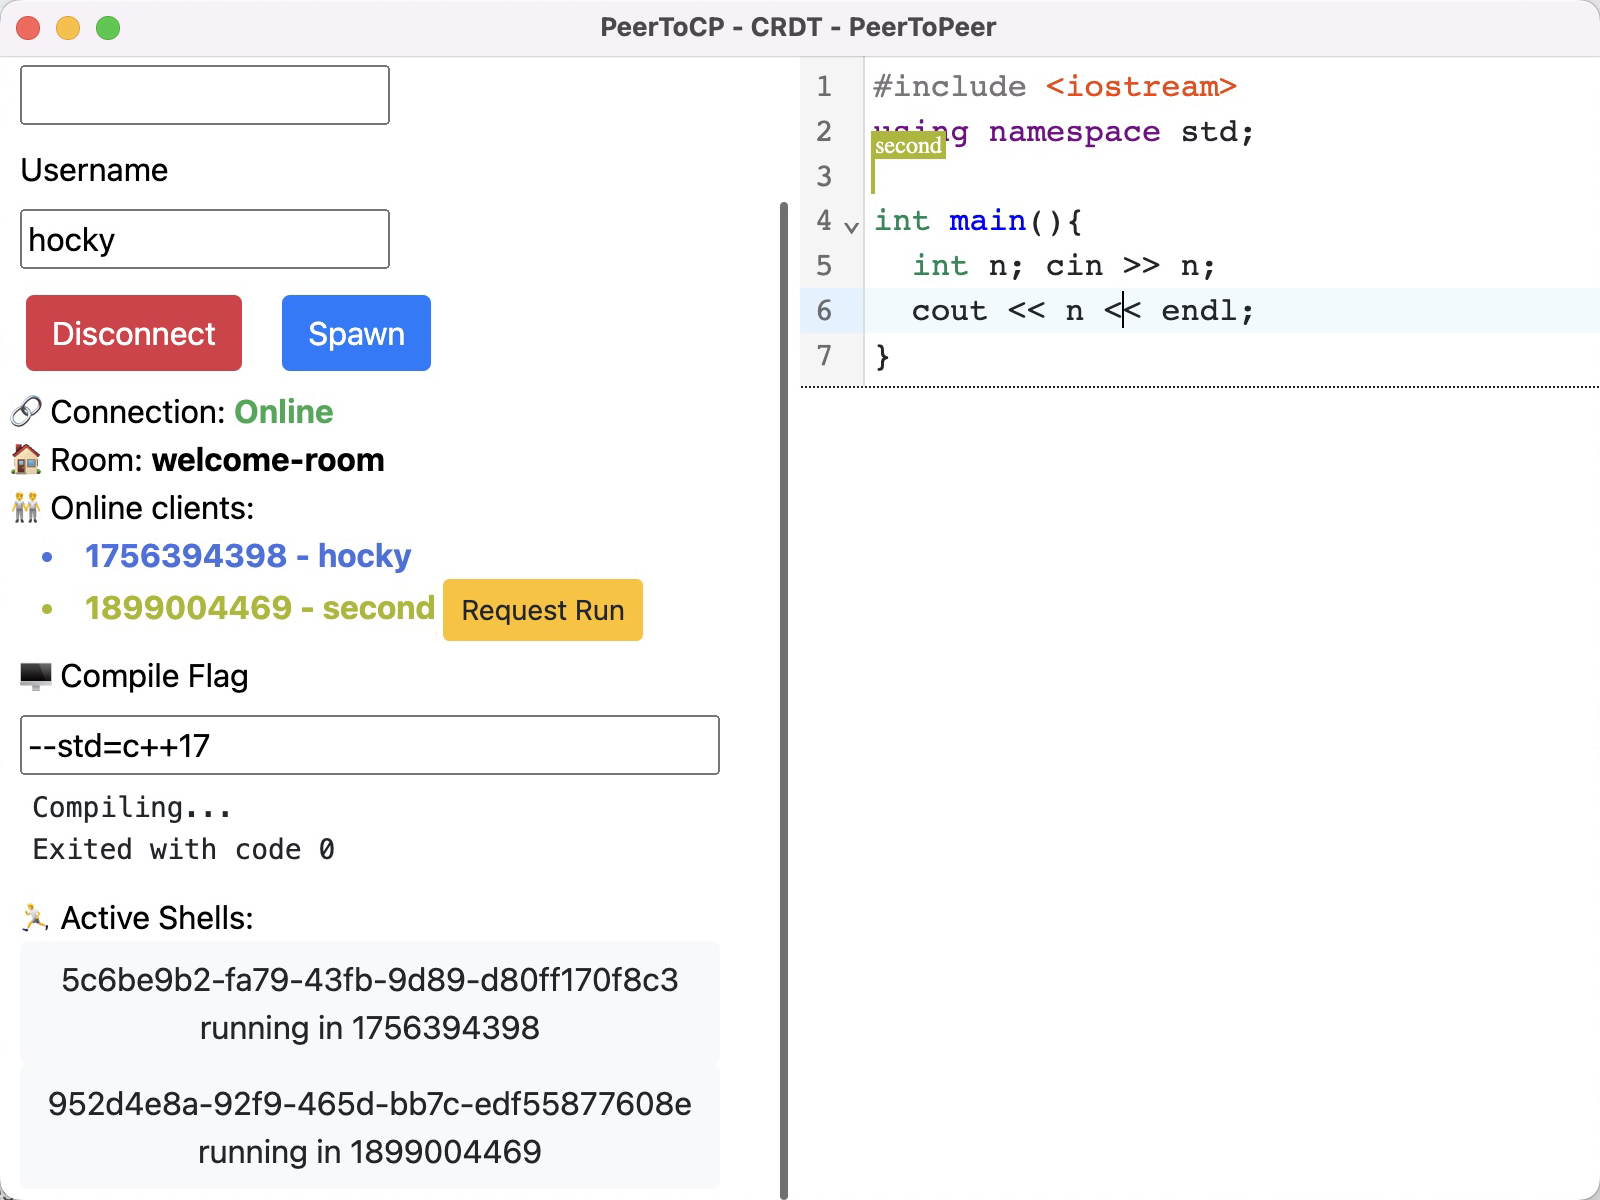
\includegraphics[width=0.82\linewidth]{figures/app-main-window}\\[0.6em]
    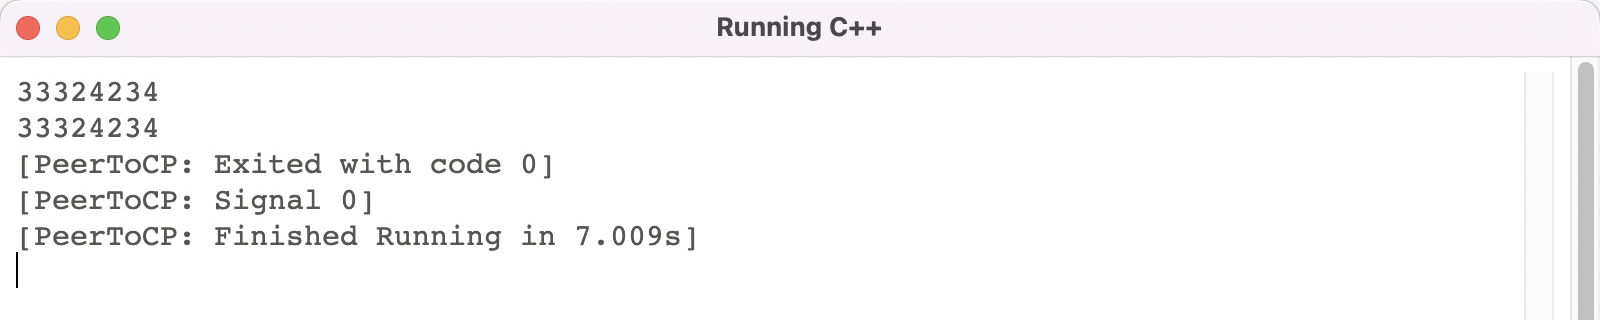
\includegraphics[width=0.82\linewidth]{figures/app-shared-shell}
    \caption[PeerToCP, peer-to-peer CRDT variant]{PeerToCP, peer-to-peer CRDT variant. Top: the main window, with the connection, the room, the online clients (each with a Request Run button), the compiler flags and the list of active shells on the left, and the shared code editor on the right, where another user's cursor, labeled \emph{second}, is visible. Bottom: a shared shell window running a compiled C++ program.}
    \label{fig:4:app}
\end{figure}

\begin{figure}[htbp]
    \centering
    % Activity diagram of the application usage flow (English redraw of
% assets/skripsi/Activity_Diagram.pdf). Three swimlanes: User A, User A's
% System, User B's System. TikZ libraries: arrows.meta, shapes.geometric.
\definecolor{actLaneUserA}{HTML}{DAE8FC}%
\definecolor{actLaneSysA}{HTML}{F8CECC}%
\definecolor{actLaneSysB}{HTML}{FFF2CC}%
\begin{tikzpicture}[
  font=\sffamily\footnotesize,
  >={Stealth[length=2mm,width=1.6mm]},
  flow/.style={->, line width=0.5pt},
  act/.style={draw, rounded corners=3pt, align=center, text width=#1,
    inner sep=2.5pt, minimum height=0.7cm, fill=white,
    execute at begin node={\hyphenpenalty=10000}},
  act/.default=2.3cm,
  dec/.style={draw, diamond, aspect=#1, inner sep=0.5pt, align=center, fill=white},
  merge/.style={draw, diamond, minimum size=0.6cm, inner sep=0pt, fill=white},
  bar/.style={fill=black, inner sep=0pt, minimum height=3.5pt, minimum width=#1},
  guard/.style={fill=white, inner sep=1.5pt},
]
  % ---- swimlanes ---------------------------------------------------------
  \def\laneA{8.9}   \def\laneB{11.9}   \def\laneEnd{15.95}
  \def\headTop{0}   \def\headBot{-0.6} \def\laneBot{-18.25}
  \fill[actLaneUserA] (0,\headTop) rectangle (\laneA,\headBot);
  \fill[actLaneSysA] (\laneA,\headTop) rectangle (\laneB,\headBot);
  \fill[actLaneSysB] (\laneB,\headTop) rectangle (\laneEnd,\headBot);
  \draw (0,\headTop) rectangle (\laneEnd,\laneBot);
  \draw (0,\headBot) -- (\laneEnd,\headBot);
  \draw (\laneA,\headTop) -- (\laneA,\laneBot);
  \draw (\laneB,\headTop) -- (\laneB,\laneBot);
  \begin{scope}[every node/.style={font=\sffamily\footnotesize\bfseries, inner sep=0pt,
      text height=1.6ex, text depth=0.4ex}]
    \node at ({\laneA/2},-0.3) {User A};
    \node at ({(\laneA+\laneB)/2},-0.3) {User A's System};
    \node at ({(\laneB+\laneEnd)/2},-0.3) {User B's System};
  \end{scope}

  % ---- User A ------------------------------------------------------------
  \node[circle, fill=black, minimum size=0.42cm, inner sep=0pt] (start) at (1.6,-1.05) {};
  \node[act=1.9cm] (open) at (1.6,-2.0) {Open the application};
  \node[act] (room) at (1.6,-3.75) {Join a room (the default room when the app first opens)};
  \node[dec=1.6] (conn) at (5.0,-3.75) {Connected to\\the server?};
  \node[act=2.4cm] (access) at (4.4,-6.15) {Access the code document and view the list of program shells};
  \node[act=1.9cm] (edit) at (1.6,-6.95) {Edit the document};
  \node[merge] (d2) at (4.4,-8.0) {};
  \node[act=2.1cm] (send) at (7.3,-8.0) {Send a compilation request with the Request Run button};
  \node[act] (switch) at (1.6,-9.75) {Switch rooms or change display name};
  \node[act=1.9cm] (close) at (7.3,-9.85) {Close the application};
  \node[circle, draw, line width=0.6pt, minimum size=0.5cm, inner sep=0pt] (end) at (7.3,-11.05) {};
  \fill (end) circle (0.15cm);
  \node[act=2.4cm] (openshell) at (4.4,-11.05) {Open one of the program shells};
  \node[merge] (d3) at (4.4,-12.45) {};
  \node[act=2.1cm] (closeshell) at (7.3,-12.45) {Close the shell};
  \node[act=1.9cm] (input) at (4.4,-14.05) {Type input into the shell};
  \node[act=2.1cm] (receive) at (7.3,-14.05) {Receive the compilation result message};

  % ---- User A's System ---------------------------------------------------
  \node[act=2.1cm] (sync) at (10.4,-3.75) {Synchronize program shells and documents};

  % ---- User B's System ---------------------------------------------------
  \node[act=1.6cm] (compile) at (13.6,-8.0) {Compile};
  \node[bar=2.7cm] (fork) at (13.4,-8.85) {};
  \node[dec=1.25] (ok) at (13.6,-10.5) {Compilation\\succeeded?};
  \node[act=2.5cm] (run) at (13.6,-12.45) {Run the program};
  \node[act=2.4cm] (add) at (13.6,-13.75) {Add to the list of running program shells};
  \node[merge] (d5) at (13.6,-15.0) {};
  \node[bar=2.7cm] (join) at (13.4,-15.7) {};
  \node[act=2.8cm] (process) at (13.6,-17.15) {Process keystroke input from any client in the program shell};

  % ---- edges -------------------------------------------------------------
  \draw[flow] (start) -- (open);
  \draw[flow] (open) -- (room);
  \draw[flow] (room) -- (conn);
  \draw[flow] (conn) -- node[guard, above] {Yes} (sync);
  \draw[flow] (conn.south) -- node[guard, right] {No} (conn.south |- access.north);
  \draw[flow] (sync.south) |- ([yshift=0.3cm]access.east);
  \draw[flow] (access) -- (d2);
  \draw[flow] (d2.west) -| (edit.south);
  \draw[flow] (edit.north) |- (conn.south west |- 0,-5.0) -- (conn.south west);
  \draw[flow] (d2) -- (send);
  \draw[flow] (d2.south west) -- (switch.north east);
  \draw[flow] (switch.west) -- (0.18,-9.75) |- (0.9,-4.85) -- (0.9,-4.85 |- room.south);
  \draw[flow] (d2.south east) -- (close.north west);
  \draw[flow] (close) -- (end);
  \draw[flow] (d2) -- (openshell);
  \draw[flow] (openshell) -- (d3);
  \draw[flow] (d3) -- (closeshell);
  \draw[flow] (closeshell.east) -| (8.7,-6.45) -- ([yshift=-0.3cm]access.east);
  \draw[flow] (d3) -- (input);
  \draw[flow] (input.south) |- (process.west);
  % The Request Run line jumps over the close-shell line.
  \draw[flow] (send.east) -- (8.58,-8.0) arc[start angle=180, end angle=0, radius=0.12] -- (compile.west);
  \draw[flow] (compile) -- (compile |- fork.north);
  \draw[flow] (fork.south -| ok.north) -- (ok.north);
  \draw[flow] (fork.south -| 12.25,0) |- (10.4,-9.25) |- (7.3,-13.1) -- (receive.north);
  \draw[flow] (ok) -- node[guard, right] {Yes} (run);
  \draw[flow] (ok.east) -| (15.15,-15.0) -- (d5.east);
  \node[guard] at (15.15,-11.9) {No};
  \draw[flow] (run) -- (add);
  \draw[flow] (add) -- (d5);
  \draw[flow] (d5) -- (d5 |- join.north);
  \draw[flow] (receive.south) |- (12.3,-15.3) -- (join.north -| 12.3,0);
  \draw[flow] (join.south -| 14.45,0) |- (15.45,-16.0) |- (conn.north east |- 0,-1.3) -- (conn.north east);
  \draw[flow] (process.east) -| (15.75,-1.0) -| (conn.north);
\end{tikzpicture}%

    \caption{How the application is used: a high-level activity diagram.}
    \label{fig:activity}
\end{figure}

When users open the application, they join the default room. They can edit the document, and synchronization runs continuously with the publish-subscribe pattern, so updates from other users arrive without having to be checked for, or polled. A user can compile and run the code on their own machine (the \emph{Spawn} button), or send a compilation request to any other user in the network (\emph{Request Run}). PeerToCP delivers the request to the chosen user without involving the other users in the network. The recipient's system compiles the code, runs the program, and adds a shell running it, with its own ID, to the list of shells that every client in the network can access. This list of shells and their contents is stored as a JavaScript object. Figure~\ref{fig:4:request-run} shows this exchange.

\begin{figure}[htbp]
    \centering
    % Request Run and a shared shell: a sequence diagram with three users, B the
% host that compiles and runs the program. Time flows down.
% TikZ libraries: arrows.meta. Colors from thesis.sty.
\begin{tikzpicture}[
  font=\sffamily\footnotesize,
  head/.style={draw=accent, fill=accentlight, line width=0.6pt, rounded corners=2pt,
    minimum width=2.3cm, minimum height=0.75cm, inner sep=2pt,
    font=\sffamily\small\bfseries, align=center},
  life/.style={draw=rulegray, line width=0.6pt},
  msg/.style={line width=0.6pt, -{Stealth[length=2.2mm,width=1.6mm]}},
  rep/.style={msg, accent},
  lab/.style={above, inner sep=1.5pt},
  act/.style={draw=rulegray, fill=codebg, line width=0.6pt, rounded corners=2pt,
    inner sep=2.5pt, minimum height=0.5cm},
  stepnum/.style={circle, fill=accent, text=white, font=\sffamily\scriptsize\bfseries,
    inner sep=0pt, minimum size=4mm},
]
  % ---- lifelines -------------------------------------------------------
  \def\xA{0}  \def\xB{5.2}  \def\xC{10.4}  \def\xN{-1.8}
  \def\yEnd{-6.6}
  \foreach \x in {\xA,\xB,\xC} \draw[life] (\x,-0.375) -- (\x,\yEnd);
  \node[head] at (\xA,0) {User A};
  \node[head] at (\xB,0) {User B (host)};
  \node[head] at (\xC,0) {User C};

  % ---- 1. A asks B to run the code ----------------------------------------
  \node[stepnum] at (\xN,-1.0) {1};
  \node[act] at (\xA,-1.0) {\emph{Request Run} for B};
  \draw[msg] (\xA,-1.65) -- node[lab] {run request (code, flags)} (\xB,-1.65);

  % ---- 2. B compiles --------------------------------------------------------
  \node[stepnum] at (\xN,-2.3) {2};
  \node[act] at (\xB,-2.3) {compile with \texttt{g++}};

  % ---- 3. B runs it in a new shell -------------------------------------------
  \node[stepnum] at (\xN,-2.95) {3};
  \node[act] at (\xB,-2.95) {spawn shell (\texttt{node-pty})};

  % ---- 4. the new shell is shared ------------------------------------------
  \node[stepnum] at (\xN,-3.6) {4};
  \node[act] at (\xB,-3.6) {add the shell to the shell list};
  \draw[rep] (\xB,-4.25) -- node[lab] {shell list update} (\xA,-4.25);
  \draw[rep] (\xB,-4.25) -- node[lab] {shell list update} (\xC,-4.25);
  \fill[accent] (\xB,-4.25) circle (1.4pt);

  % ---- 5. C types into the shell -------------------------------------------
  \node[stepnum] at (\xN,-4.9) {5};
  \draw[msg] (\xC,-4.9) -- node[lab] {keystroke} (\xB,-4.9);

  % ---- 6. the program's output is replicated --------------------------------
  \node[stepnum] at (\xN,-5.55) {6};
  \node[act] at (\xB,-5.55) {append the output to the shell's array};
  \draw[rep] (\xB,-6.2) -- node[lab] {shell output} (\xA,-6.2);
  \draw[rep] (\xB,-6.2) -- node[lab] {shell output} (\xC,-6.2);
  \fill[accent] (\xB,-6.2) circle (1.4pt);

  % ---- note ------------------------------------------------------------------
  \node[draw=rulegray, fill=codebg, line width=0.6pt, rounded corners=2pt, inner sep=3pt,
    font=\sffamily\footnotesize\itshape, text=black!70] at (\xB,-7.1)
    {peer-to-peer: messages go directly between peers; client-server: via the server};
\end{tikzpicture}%

    \caption[Running a program on another user's machine]{Running a program on another user's machine. User A asks user B to run the code; B compiles it, runs it in a new shell and shares that shell with everyone. Keystrokes from any user go to B, the host, and the program's output is replicated to all users. In the peer-to-peer variant the messages travel directly between peers; in the client-server variants they go through the server.}
    \label{fig:4:request-run}
\end{figure}

In Figure~\ref{fig:activity}, how the program shells and the document are synchronized depends on the variant. In the client-server architecture, user A's application connects to and synchronizes with the server; in the peer-to-peer architecture, it connects to and synchronizes with the other peers directly. Likewise, compilation requests and the messages carrying compilation results go directly between peers in the peer-to-peer architecture, but must go through the server in the client-server architecture.

\section{Peer-to-Peer and Client-Server CRDT Variants}
\label{sec:desain_crdt}

Both CRDT variants use the Yjs library. Every peer or client holds a replica, a \texttt{Y.Doc}, which can contain several nested CRDTs. The code is a \texttt{Y.Text}, and the shells are a \texttt{Y.Map} that maps the ID of each shell to a \texttt{Y.Array} holding its contents. The peer-to-peer variant uses the y-webrtc network provider, modified with an interface for sending a message to a specific peer over an RTCDataChannel (Figure~\ref{crdt-p2p}). A keystroke typed by any peer is sent directly to the host peer running the program, which appends the program's response to the array of that shell.

\begin{figure}[htbp]
    \centering
    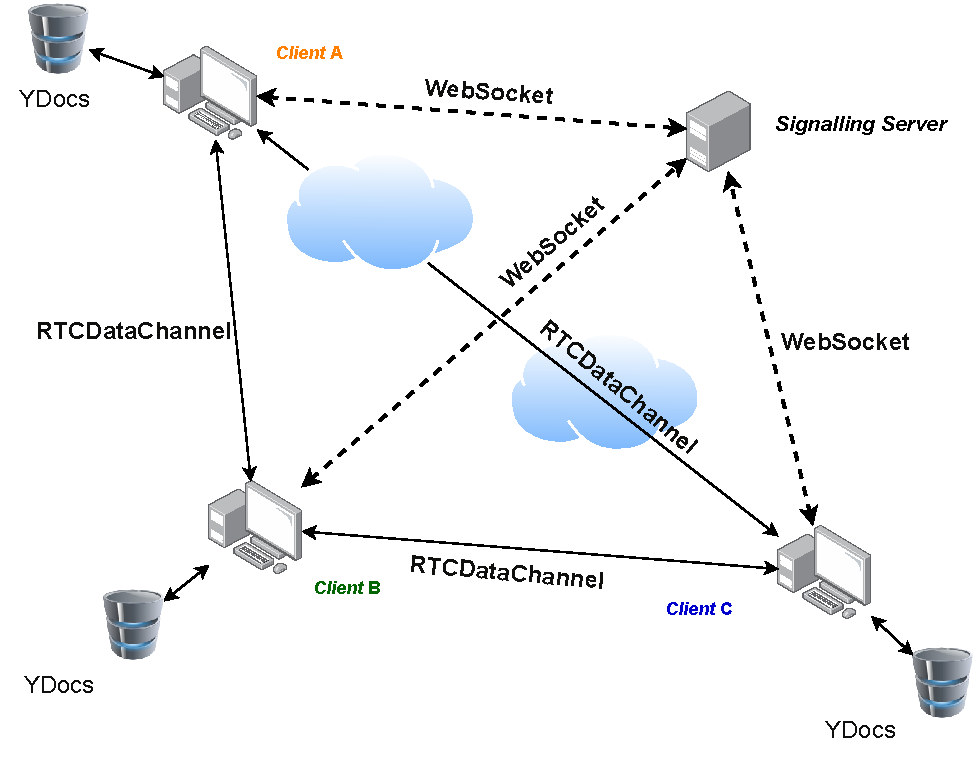
\includegraphics[scale=0.62]{figures/arch-crdt-p2p}
    \caption[The peer-to-peer CRDT variant]{The peer-to-peer CRDT variant: every client keeps a Yjs replica and is connected to every other client over WebRTC data channels; a WebSocket signaling server only introduces the peers to each other.}
    \label{crdt-p2p}
\end{figure}

\begin{figure}[htbp]
    \centering
    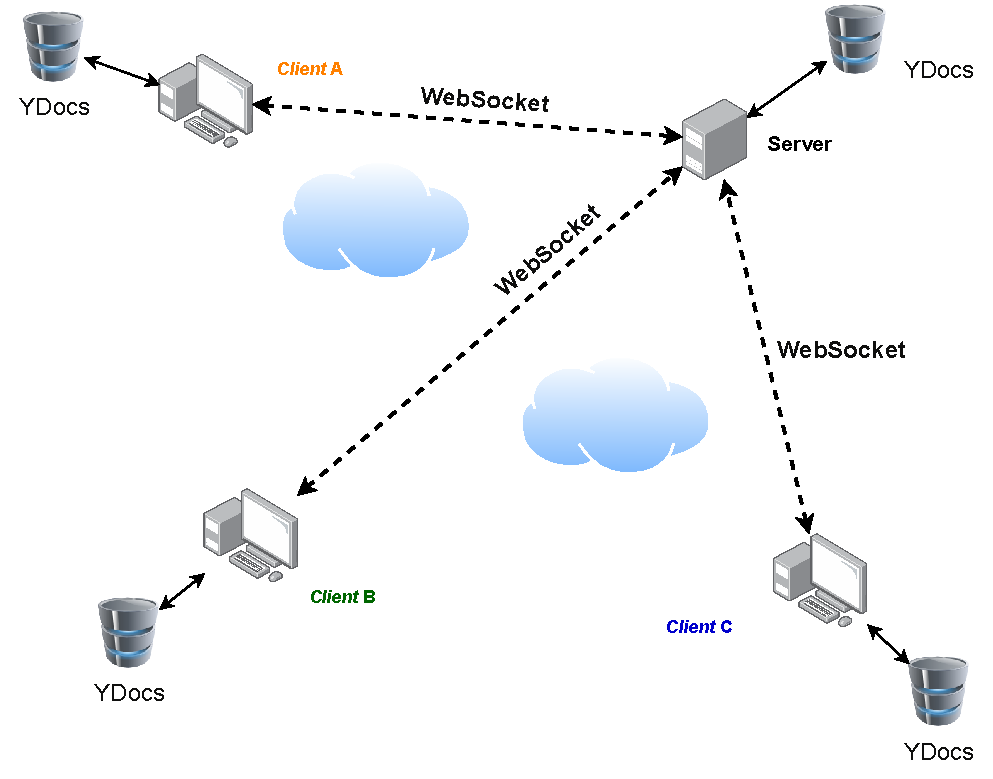
\includegraphics[scale=0.62]{figures/arch-crdt-cs}
    \caption[The client-server CRDT variant]{The client-server CRDT variant: every client keeps a Yjs replica and synchronizes it over WebSocket with the server, which keeps a replica of its own.}
    \label{crdt-cs}
\end{figure}

The two CRDT variants differ only in their network provider. The client-server variant (Figure~\ref{crdt-cs}) uses y-websocket, also modified so that it can send a message to a specific client through the server. A network provider gives every peer or client in a distributed network an abstraction for communicating with the others. In the client-server architecture, the server adds one feature: persistence. The server keeps its own replica of the document, so the document survives even when no client is connected. Besides CRDTs, the client-server architecture is also used with operational transformation, in the third variant compared in this study, whose OT satisfies only TP1.

\section{Client-Server Operational Transformation Variant}
\label{sec:design_ot}

For a document that holds only plain text, operational transformation that satisfies only TP1 can be implemented simply on a client-server architecture. This variant uses the @codemirror/collab library, which implements operational transformation and represents CodeMirror changes as deltas. The client keeps an array of local changes the server does not yet know about. It sends these changes periodically, together with the latest server version it has applied, through RPC over WebSocket; the RPC call does not block the client while it waits for the reply, before the next attempt to send. If the server already has a newer version than the one the changes are based on, it rejects them and tells the client to rebase: to apply the server's newer updates first, before trying again.

\begin{figure}[htbp]
    \centering
    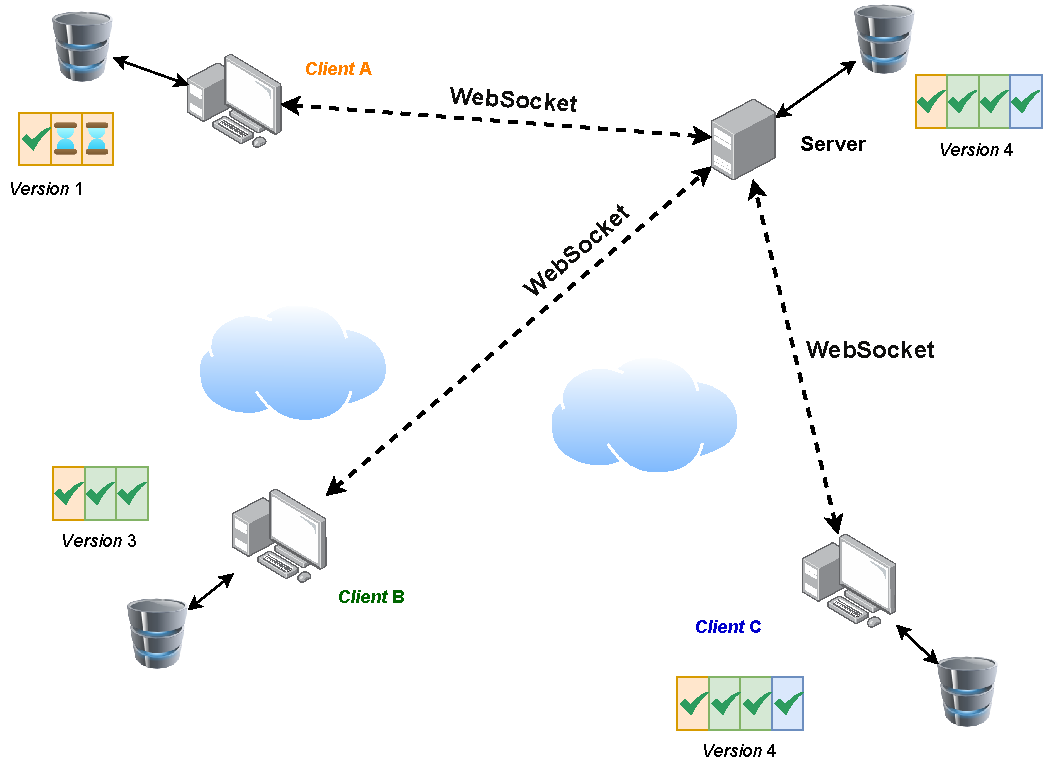
\includegraphics[width=11cm]{figures/arch-ot-cs}
    \caption[The client-server OT variant]{The client-server OT variant: the server holds the authoritative sequence of versions, and each client keeps its pending local changes until the server accepts them.}
    \label{fig:websocket_ot}
\end{figure}

Remote changes received from the server are transformed against the local changes the server does not know about yet; the local changes are then replaced by their versions transformed against the remote ones, and these are what the client sends next. Operational transformation happens only on the clients, and the server applies changes strictly in order, so every replica of the document converges to the same text. Figure~\ref{fig:websocket_ot} shows this architecture.

\begin{figure}[htbp]
    \centering
    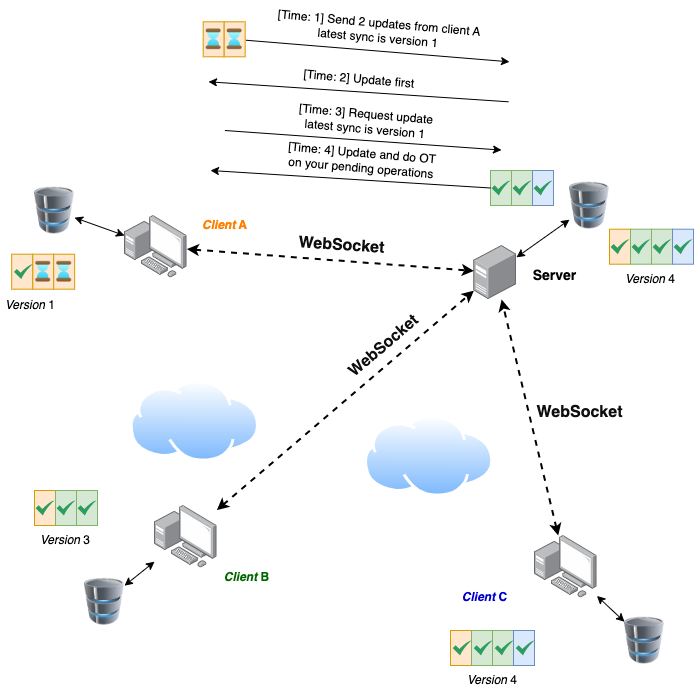
\includegraphics[width=7cm]{figures/ot-sync-1}\hfill
    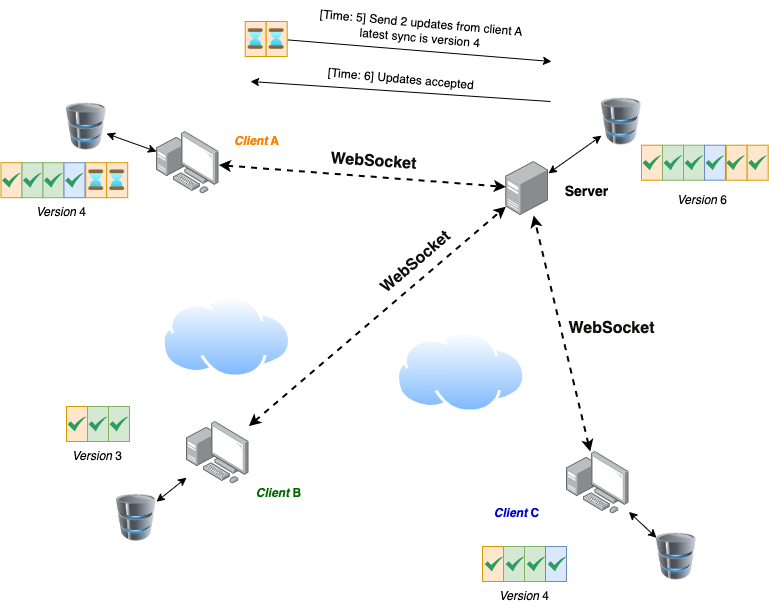
\includegraphics[width=7cm]{figures/ot-sync-2}
    \caption[Synchronization in the OT variant]{Synchronization in the OT variant. Left: client A's two pending updates are rejected, because the server has moved on. Right: after pulling the server's new operations and transforming its own against them, client A's updates are accepted.}
    \label{fig:ots}
\end{figure}

Figure~\ref{fig:ots} shows an example. The server cannot accept client A's two pending updates until client A has all of the server's latest versions. After pulling updates and receiving three new operations from the server, client A transforms its two pending updates against them. Client A's local document is now at version~4, and it can send its updates. The server appends client A's two operations, which brings it to version~6.

The shells of running programs work the same way. When a client types a keystroke into one of the active shells, the keystroke is sent through a similar mechanism, but routed to the client that hosts, that is, runs, the program. The host sends the changes to the shell to the server periodically, as long as there are changes the server has not received, and when a change arrives the server notifies every client to pull it. Because only the host produces the shell's contents, these updates need no transformation function, unlike plain-text OT. Positions need no mapping either, because the cursor is always after the last character. Applying updates serially in this way prevents race conditions during network disruptions.

\section{Evaluation Design}
\label{sec:desain_evaluasi}

The three architectures are back ends for the same editor interface, so the benchmark measures, end to end, what users experience. It consists of scenarios that cover the aspects being tested, run under conditions kept as identical as possible across the variants.

The system is evaluated on the Compute Engine service of Google Cloud Platform. Each variant has its server on an instance in the \texttt{asia-southeast1-b} zone, on an \texttt{e2-medium} machine with 2~vCPUs, 4~GiB of RAM and Debian~11. This machine type was chosen so that the server's specifications do not limit the benchmark. No relay (TURN) server is provided for peers that cannot connect to each other in the peer-to-peer variant: the study assumes that the WebRTC connections between peers can always be set up.

The users are \texttt{e2-small} virtual machines with 2~vCPUs, 2~GiB of RAM and Debian~11, all in the \texttt{asia-southeast2-a} zone, a region close to the servers, to approximate real-world use of PeerToCP. Four test scenarios are run, each with $n \in \{2, 4, 8\}$ users, to show how the system scales with the number of users in a network. The largest value of $n$ reflects the expected maximum number of users of PeerToCP, which is no more than eight. Table~\ref{tab:skenarios} summarizes the scenarios.

\begin{table}[htbp]
\centering
\caption{Test scenarios.}
\label{tab:skenarios}
\begin{tabular}{@{}clccc@{}}
\toprule
\textbf{Scenario} & \textbf{Component} & \textbf{Measures latency} & \textbf{Duration (s)} & \textbf{Disconnection} \\
\midrule
1 & Code editor & No  & 180            & Yes, 30\,s \\
2 & Shell       & No  & $\approx$100   & Yes, 20\,s \\
3 & Code editor & Yes & 120            & No \\
4 & Shell       & Yes & $\approx$100   & No \\
\bottomrule
\end{tabular}
\end{table}

\paragraph{Scenario 1: editing under stress.} The first scenario simulates a stream of edits in the code editor, with each number of peers $n$, for the scalability aspect. Every 100~milliseconds, for three minutes, each client performs one of three random operations, chosen with equal probability:

\begin{enumerate}
    \item inserting (\texttt{insert}) a random string of 2 to 5 characters;
    \item deleting (\texttt{delete}) a range of 1 to 3 characters;
    \item replacing (\texttt{replace}) a range of 2 to 5 characters with a random string of 2 to 5 characters.
\end{enumerate}

On each client, these operations grow the document by about 5 characters per second on average, and change about 41.67 characters per second, insertions and deletions together. The tests start at the same time on every client, using the operating system's clock, which is synchronized by default. Some error between the clocks is unavoidable and is assumed to be negligible; identical instances for every client reduce the bias from differences between them. In addition, each client disconnects from the network for 30~seconds, starting at a random time between 60 and 90~seconds into the test, so that the disconnection always falls between the first and the last minute. At the end, every editor is connected again, for a final synchronization with the other users. While an editor is disconnected, it keeps performing \texttt{insert}, \texttt{delete} and \texttt{replace} operations, which tests the local-first aspect.

The first scenario is a stress test of the editing that can happen in the real world. After the test, the system waits for one minute, to give synchronization time to finish. The time of the last update is recorded and compared, for the responsiveness and scalability aspects. The hash of the final document is recorded on every client and compared across them, for the correctness aspect. The RAM, CPU and network activity of the first two clients of each run, and of the server, are recorded with the Netdata monitoring agent, for the lightweight and scalability aspects.

\paragraph{Scenario 2: a shared shell under disconnection.} The second scenario uses the same environment as the first. It tests the shell with each number of clients $n$, by running a C++ program that prints 100 random unsigned 64-bit integers, waiting a random 500 to 1500~milliseconds before each one. Meanwhile, a 20-second network disconnection starts at a random time 10 to 40~seconds after the program starts. As in the first scenario, the last synchronization time, the device activity and the hash of every shell on every client are recorded and compared, to make sure that every user ends up with the same shell replica.

\paragraph{Scenarios 3 and 4: latency.} The last two scenarios measure the latency of the code editor and of the shell, respectively. In the third scenario, the $n$ peers are set up as before, and each performs two kinds of operation: inserting a timestamp into the editor, and replacing a range of 10 to 15 characters with a timestamp. Each operation waits a random 500 to 1000~milliseconds, so that the operations do not all happen at a fixed period. Every client captures the timestamps it receives and measures the latency as the time between a timestamp being written and its arrival at another client. In the fourth scenario, every client runs a C++ program that prints 100 timestamps, with a random delay of 500 to 1500~milliseconds between them. Every client captures each timestamp and measures its latency in the same way, as the time between the host of the shell (the user running the program) adding the timestamp and each other user receiving it. Scenarios 3 and 4 have no disconnections, so that the data for the responsiveness aspect are as accurate as possible.
